\documentclass[t]{beamer}
\usetheme[deutsch]{KIT}
\setbeamercovered{transparent}
\setbeamertemplate{navigation symbols}{}

\KITfoot{Tutoriumsmaterial von Joachim Priesner, Sebastian Ullrich und Max Wagner \hspace{2.5cm} Basierend auf den Folien von Simon Stroh und Moritz v. Looz}
\usepackage[utf8]{inputenc}
\usepackage{amsmath}
\usepackage{ifthen}
\usepackage{amssymb}
\usepackage{tikz}
\usepackage{ngerman}
\usetikzlibrary{automata}
\usenavigationsymbols


\title{Theoretische Grundlagen der Informatik}
\subtitle{Tutorium}
\author{Moritz von Looz, Simon Stroh}

\institute[ITI]{Institut für Theoretische Informatik}

\TitleImage[height=\titleimageht]{images/tmaschine.png}

\newcommand{\N}{\ensuremath{\mathbb{N}}}
\newcommand{\M}{\ensuremath{\mathcal{M}}}
\newcommand{\classP}{\ensuremath{\mathcal{P}}}
\newcommand{\classNP}{\ensuremath{\mathcal{NP}}}
\newcommand{\co}{\ensuremath{\mathsf{co\text{-}}}}
\newcommand{\pot}{\ensuremath{\mathcal{P}}}
\newcommand{\abs}[1]{\ensuremath{\left\vert #1 \right\vert}}
\newcommand{\menge}[2]{\ensuremath{\left\lbrace #1 \,\middle\vert\, #2 \right\rbrace}}
\newcommand{\ducttape}[1]{\vspace{#1}}
\newcommand{\neglit}[1]{\overline{#1\vphantom{x^a}}}
\newcommand{\recipe}{\raisebox{-.3cm}{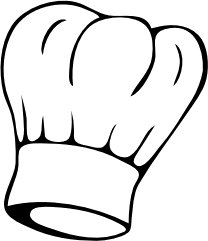
\includegraphics[scale=.15]{images/chefs-cap.png}}\hspace{0.2cm}}

\newcommand{\invincible}{\setbeamercovered{invisible}} %  "Yesss! I am invincible!!" (Boris Grishenko)
\newcommand{\vincible}{\setbeamercovered{transparent}}

% \@ifundefined{tikzset}{}{\tikzset{initial text=}} % Text "start" bei Startknoten unterdrücken
\tikzstyle{every node}=[thick]
\tikzstyle{every line}=[thick]

\newcommand{\tutnr}[1]{
  \subtitle{Tutorium #1}
	\begin{frame}
		\maketitle
	\end{frame}
}

\newcommand{\uebnr}[1]{
  \subtitle{Anmerkungen zum #1. Übungsblatt}
	\begin{frame}
		\maketitle
	\end{frame}
}

\begin{document}


% Greibach-Normalform
\subsection{Greibach-Normalform}
\begin{frame}
\frametitle{Greibach Normalform}
\begin{exampleblock}{Definition}
Eine kontextfreie Grammatik ist in \textbf{Greibach-Normalform}, wenn alle Ableitungsregeln von der Form 
$$ A \rightarrow a\alpha \text{ mit } A \in V\text{,} a\in \Sigma \text{ und } \alpha \in V^*$$
sind.
\end{exampleblock}
\end{frame}

\begin{frame}
\frametitle{Zur Greibach-Normalform}
\begin{itemize}
\item Weitere Normalform für CH-2 Grammatiken, d.h. jede Grammatik kann in Greibach-Normalform gebracht werden
\item Zur Konstruktion von Kellerautomaten aus Grammatiken
\item Es kann stärker, aber äquivalent, verlangt werden, dass auf der rechten Seite höchstens zwei Variablen vorkommen.
\end{itemize}
\end{frame}

\begin{frame}
\frametitle{Umwandlung in Greibach-Normalform}
\begin{exampleblock}{Nebenbemerkung}
Im folgenden stehen Kleinbuchstaben für Terminale, Großbuchstaben für einzelne Nichtterminale und griechische Buchstaben für (eventuell) mehrere Nichtterminale 
\end{exampleblock}
Die Grammatik sei zunächst in Chomsky-Normalform.
\end{frame}

\begin{frame}
\frametitle{Annahmen}
\begin{block}{Annahmen}
\begin{itemize}
 \item Wir gehen davon aus, dass die Grammatik $G$ in Chomsky-Normalform ist, mit $V = \{A_1 ... A_m \}$ und $\Sigma = \{\alpha_1 ... \alpha_n\}$
 \item Folglich sind alle Regeln von der Form $A_i \rightarrow A_jA_k$ oder $A_i \rightarrow \alpha_j$
\end{itemize}
\end{block}
\end{frame}

\begin{frame}
\frametitle{Schritt 1}
Es gebe die Nichtterminale $\{A_0, \ldots, A_N\}$
\begin{enumerate}
\item für alle $i$ in $1, \ldots, N$
\begin{enumerate}
\item für alle $j$ in $1, \ldots, i$
\begin{enumerate}
\item Simuliere alle Regeln für $A_j$ bei Produktionen der Form $A_i \rightarrow A_j\alpha$ mit $j < i$ auf der rechten Seite.
\item für Produktionen der Form $A_i \rightarrow A_i\alpha$ führe eine neue Variable ein (wie: siehe nächste Folie).
\end{enumerate}
\end{enumerate}
\end{enumerate}
\end{frame}

\begin{frame}
\frametitle{$A_i \rightarrow A_i\alpha$}
Für Regeln der Form 
$$A \rightarrow A\alpha_1 \mid \ldots \mid A\alpha_r$$
$$A \rightarrow \beta_1 \mid \ldots \mid \beta_s$$
(wobei $\beta_i$ nicht mit $A$ beginnt) führe ein neues Nichtterminal $\beta$ ein. Ersetze nun die Regeln
$$A \rightarrow A\alpha_1 \mid \ldots \mid A\alpha_r$$
durch
$$A \rightarrow \beta_1B \mid \ldots \mid \beta_sB$$
$$B \rightarrow \alpha_1 \mid \ldots \mid \alpha_r$$
$$B \rightarrow \alpha_1B \mid \ldots \mid \alpha_rB$$
\end{frame}

\begin{frame}
 \frametitle{Schritt 2}
Gehen nun die Produktionen absteigend nach $k$ sortiert durch und simuliere bei alle Regeln mit $A_k \rightarrow A_j\alpha$ die Produktionen für $A_j$ auf der rechten Seite.\\
Da alle Regeln, die mit einem $A_i$ anfangen, der Greibach-Normalform genügen, kann man dieses Verfahren nun bei den neuen Regeln für $B_1,\ldots$ auch anwenden, danach ist die Grammatik in Greibach-Normalform.
\end{frame}

\begin{frame}
\frametitle{Aufgabe zur Greibach-Normalform}
Sei die Grammatik $G$ gegeben durch
\begin{itemize}
 \item $\Sigma = \{0, 1\}$
 \item $V = \{A_1, A_2, A_3\}$
 \item $S = A_1$
 \item $R = \{A_1 \rightarrow A_2A_3, A_2 \rightarrow A_3A_1, A_2 \rightarrow 1, A_3 \rightarrow A_1A_2, A_3 \rightarrow 0\}$
\end{itemize}

Bringen Sie $G$ in Greibach-Normalform.

\textbf{Lösung:} Siehe Skript.
\end{frame}

% Kellerautomaten
\subsection{Kellerautomat}
\begin{frame}
\frametitle{Definition}
Ein (nichtdeterministischer) \textbf{Kellerautomat} (NPDA bzw PDA, Pushdown Automaton) besteht aus $(Q, \Sigma, \Gamma, q_0, Z_0,\delta, F)$, wobei
\begin{itemize}
\item $Q$ endliche Zustandsmenge
\item $\Sigma$ endliches Eingabealphabet
\item $\Gamma$ endliches STACK-Alphabet
\item $q_0 \in Q$ Anfangszustand
\item $Z_0 \in \Gamma$ Initialisierung des STACK
\item $\delta : Q \times ( \Sigma \cup \{\varepsilon\}) \times \Gamma \rightarrow 2^{Q \times \Gamma^*}$
\begin{itemize}
\item $\delta(q, a, Z) \subseteq \{(q,\gamma) : q \in Q, \gamma \in \Gamma^*\}$
\item $\delta(q, \varepsilon, Z) \subseteq \{(q,\gamma) : q \in Q, \gamma \in \Gamma^*\}$
\end{itemize}
\item $F \subseteq Q$ Menge der akzeptierenden Endzustände, $F=\emptyset$ ist möglich.
\end{itemize}
\end{frame}

\begin{frame}
\frametitle{Zu Kellerautomaten}
\begin{itemize}
\item Akzeptieren, wenn \emph{entweder} der Stack leer ist \emph{oder} wenn der Automat in einen akzeptierenden Zustand kommt
\item Sind im allgemeinen nichtdeterministisch
\item Man kann Endzustände auch aus der Definition weglassen und alternativ verlangen, dass der Automat genau bei leerem Keller akzeptiert.
\item Man kann sogar alle Zustände bis auf einen weglassen und alles in die Kellerbelegung kodieren
\end{itemize}
\end{frame}

\begin{frame}
\frametitle{Beispiel}
$M = (Q, \Sigma, \Gamma, q_0, Z_0, \delta, F)$
\begin{itemize}
\item $Q = \{q_0, q_1, q_2\}$, $Z_0 = \{\#\}$
\item $\Sigma = \{a,b\}$
\item $\Gamma = \{\#,X\}$
\item $F = \{q_2\}$
\end{itemize}
\begin{figure}
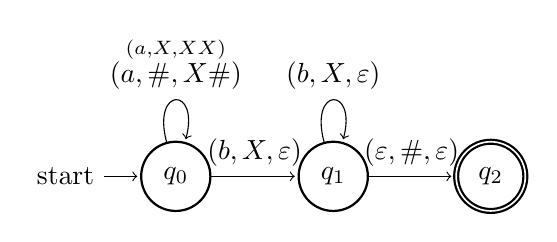
\begin{tikzpicture}[node distance=2cm,shorten >=1pt,auto]
\node[state,initial]   (q_0)                {$q_0$};
\node[state]           (q_1) [right of=q_0] {$q_1$};
\node[state,accepting] (q_2) [right of=q_1] {$q_2$};
\path[->]	(q_0) 	edge 			node {$(b,X,\varepsilon)$}				(q_1)
			edge [loop above]	node {$\stackrel{(a,X,XX)}{(a,\#,X\#)}$}	 	() %stackrel is wrong here.
		(q_1)	edge			node {$(\varepsilon,\#,\varepsilon)$}			(q_2)
			edge [loop above]	node {$(b,X,\varepsilon)$}				();
\end{tikzpicture}
\end{figure}
\end{frame}

\begin{frame}
\frametitle{Aufgaben}
\begin{itemize}
\item Welche Sprache akzeptiert der Beispielautomat der vorigen Folie?
\end{itemize}
\end{frame}

% end of ifthenelse WAY up there
}
%

\section{12. Tutoriumsvorschlag}
%TODO: Beispiel Kellerautomat
\subsection{Kellerautomat aus Greibach-Normalform}
\begin{frame}
 \frametitle{Kellerautomat aus Greibach-Normalform}
 \begin{block}{Erinnerung: Greibach-Normalform}
  Eine kontextfreie Grammatik ist in \textbf{Greibach-Normalform}, wenn alle Ableitungsregeln von der Form   
  \[ A \rightarrow a\alpha \text{ mit } A \in V\text{,} a\in \Sigma \text{ und } \alpha \in V^*\]
  sind.
 \end{block}
 \pause
 \begin{block}{Erinnerung: Übergangsfunktion des Kellerautomaten}
 Die Eingabe enthält einen Zustand, ein $a \in \Sigma \cup \{\varepsilon\}$ und ein Zeichen des Stacks.
 \[\delta : Q \times ( \Sigma \cup \{\varepsilon\}) \times \Gamma \rightarrow 2^{Q \times \Gamma^*}\]
 \vspace{-0.5cm}
 \end{block}
 \pause
 Wie könnte man mit einer Grammatik $G$ in Greibach-Normalform einen Kellerautomaten konstruieren, der $L(G)$ erkennt?
\end{frame}

\begin{frame}
 \begin{block}{Konstruktion des Kellerautomaten}
 Gegeben sei eine kontextfreie Grammatik \(G = (\Sigma, V, S, R)\) in Greibach-Normalform.\\
 Konstruiere einen Kellerautomaten \(PDA = (Q, \Sigma', \Gamma, q_0, Z_0, \delta, F)\) mit:
 \begin{itemize}
  \item $Q := \{q_0\}$
  \item $F := \emptyset$
  \item $\Sigma' := \Sigma$
  \item $\Gamma := V$
  \item $Z_0 := S$
  \item $\delta(q_0, a, A) :=  \{(q_0,\alpha) | (A \rightarrow a \alpha) \in R \}$
 \end{itemize}
 \end{block}
 \pause
 Der Automat akzeptiert durch leeren Stack.
\end{frame}

\begin{frame}
Greibach-Normalform der Aufgabe von letztem Mal:
\begin{itemize}
 \item $V=\{A_1, A_2, A_3, B_3\}$
 \item $\Sigma = A_1$
 \item $S = A_1$
 \item $R = \{A_1 \rightarrow 1A_3, A_1 \rightarrow 0B_3A_1A_3, A_1 \rightarrow 1A_3A_2A_1A_3, A_1 \rightarrow 0A_1A_3, A_1 \rightarrow 1A_3A_2B_3A_1A_3,
 A_2 \rightarrow 0B_3, A_2 \rightarrow 1A_3A_2A_1, A_2 \rightarrow 0A_1, A_2 \rightarrow 1A_3A_2B_3A_1, A_2 \rightarrow 1,
 A_3 \rightarrow 0B_3, A_3 \rightarrow 1A_3A_2B_3, A_3 \rightarrow 1A_3A_2, A_3 \rightarrow 0,
 B_3 \rightarrow 1A_3A_2A_2, B_3 \rightarrow 0B_3A_1A_3A_3A_2, B_3 \rightarrow 1A_3A_2A_1A_3A_3A_2, B_3 \rightarrow 0A_1A_3A_3A_2,
 B_3 \rightarrow 1A_3A_2B_3A_1A_3A_3A_2, B_3 \rightarrow 1A_3A_3A_2B_3, B_3 \rightarrow 0B_3A_1A_3A_3A_2B_3, B_3 \rightarrow 1A_3A_2A_1A_3A_3A_2B_3
 B_3 \rightarrow 0A_1A_3A_3A_2B_3, B_3 \rightarrow 1A_3A_2B_3A_1A_3A_3A_2B_3
 \}$
\end{itemize}
\pause
Die ursprüngliche Grammatik hatte nur fünf Regeln.
\end{frame}

\begin{frame}
 \frametitle{Kellerautomat}
\(PDA = (Q, \Sigma', \Gamma, q_0, Z_0, \delta, F)\) mit:
 \begin{itemize}
  \item $Q := \{q_0\}$
  \item $F := \emptyset$
  \item $\Sigma' := \Sigma$
  \item $\Gamma := V$
  \item $Z_0 := A_1$
  \item $\delta$ siehe nächste Folie
 \end{itemize}
 \begin{block}{Umwandlung}
 Aus \(A_1 \rightarrow 1A_3, A_1 \rightarrow 1A_3A_2A_1A_3, A_1 \rightarrow 1A_3A_2B_3A_1A_3\)
 wird \(\delta(q_0, A_1, 1) = \{(q_0, A_3), (q_0, A_3A_2A_1A_3), (q_0, A_3A_2B_3A_1A_3) \}\)
 \end{block}
\end{frame}

\begin{frame}
 \frametitle{$\delta$}
\begin{itemize}
 \item \(\delta(q_0, A_1, 0) = \{ (q_0, B_3A_1A_3), (q_0, A_1A_3)\}\)
 \item \(\delta(q_0, A_1, 1) = \{(q_0, A_3), (q_0, A_3A_2A_1A_3), (q_0, A_3A_2B_3A_1A_3) \}\)
 \item \(\delta(q_0, A_2, 0) = \{(q_0, B_3), (q_0, A_1)\}\)
 \item \(\delta(q_0, A_2, 1) = \{(q_0, A_3A_2A_1), (q_0, A_3A_2B_3A_1), (q_0, \varepsilon)\}\)
 \item \(\delta(q_0, A_3, 0) = \{(q_0, B_3), (q_0, \varepsilon)\}\)
 \item \(\delta(q_0, A_3, 1) = \{(q_0, A_3A_2B_3), (q_0, A_3A_2, A_3)\}\)
 \item $\delta(q_0, B_3, 0) = \{(q_0, B_3A_1A_3A_3A_2), (q_0, A_1A_3A_3A_2), (q_0, B_3A_1A_3A_3A_2B_3),$ $ (q_0, A_1A_3A_3A_2B_3)\}$
 \item \(\delta(q_0, B_3, 1) = \{(q_0, A_3A_2A_2), (q_0, A_3A_2A_1A_3A_3A_2), (q_0, A_3A_2B_3A_1A_3A_3A_2),$ $
 (q_0, A_3A_3A_2B_3), (q_0, A_3A_2A_1A_3A_3A_2B_3), (q_0, A_3A_2B_3A_1A_3A_3A_2B_3)\}\)
\end{itemize}
\end{frame}

\begin{frame}
 \frametitle{Tripelkonstruktion}
 \begin{itemize}
  \item Umkehrung der Konstruktionsrichtung
  \item Aus einem PDA $\mathcal{A} = (Q, \Sigma, \Gamma, \delta, q_0, Z_0)$ wird eine Grammatik \textit(G) mit $L_{\mathcal{A}} = L(G)$ erzeugt.
 \end{itemize} 
 \begin{itemize}
  \item $V := \{[q, X, p]p, q \in Q, X \in \Gamma \} \cup S$
  \item $R := $
  \begin{itemize}
   \item $S \rightarrow [q_0, Z_0, q]$ für alle $q \in Q$
   \item $[q, X, q_{m+1}] \rightarrow a[q_1, Y_1, q_2] ... [q_m, Y_m, q_{m+1}]$ für alle $q_2$, ..., $q_{m+1} \in Q$,
   falls $(q_1, Y_1, ..., Y_m) \in \delta(q, a, X)$
  \end{itemize}
 \end{itemize}

\end{frame}

%TODO: Beispiel Tripelkonstruktion

\begin{frame}
 \frametitle{Wiederholung Chomsky-Hierarchie}
 $u \in V^+$, $v \in (\Sigma \cup V)$, $A \in V$, $a \in \Sigma$.
  Ausnahme: S kommt bei Chomsky-1-Grammatiken nicht auf rechten Seiten vor.
 \begin{table}
 \begin{center}
 \begin{tabular}{| l | c | p{1.4cm} | c | c | c | l |}
 \hline
 & & & \multicolumn{3}{|c|}{Abgeschlossen} &\\
 Typ & Bezeichnung & Regeln & $\cup$ & $\cap$ & $\cdot$ & Modell\\ \hline
 0 & semientscheidbar & alles & ja & ja & ja & TM \\ \hline
 1 & kontextsensitiv & $u \rightarrow v$ $|u| \leq |v|$ & ja & ja & ja &  LBA \\ \hline
 2 & kontextfrei & $A \rightarrow v$ & ja & nein & ja & Kellerautomat \\ \hline
 3 & regulär & $A \rightarrow a$  $A \rightarrow aB$ & ja & ja & ja & endlicher Automat \\ \hline
 \end{tabular}
 \end{center}
 \end{table}
\pause
Welche dieser Sprachenklassen sind unter der Komplementbildung abgeschlossen?
\end{frame}

\begin{frame}
 \frametitle{Anmerkung zum aktuellen Übungsblatt}
 Die Greibach-Normalform muss nicht mit der Methode aus dem Skript erzeugt werden,
 die Anwendungsreihenfolge der Regeln (i) und (ii) kann selbst gewählt werden.
\end{frame}

\section{13. Tutoriumsvorschlag}
\begin{frame}
Geben Sie einen zu folgendem NEA äquivalenten DEA an:

\begin{center}
 \includegraphics[width=5cm]{NEA}
\end{center}
\end{frame}

\begin{frame}
Beweisen Sie die $\mathcal{NP}$-Vollständigkeit des Problems HITTING SET:
\begin{quote}
  Gegeben eine Menge $M$ und eine Menge $T$ von Teilmengen von $M$,
  $K \in \mathbb{N}$. Gibt es eine Teilmenge $M' \subseteq M$ mit $|M'| \leq K$ so,
  dass $M'$ mindestens ein Element jeder Teilmenge $t \in T$ enthält?
\end{quote}
\textbf{Lösungshinweis:}
 Reduziere von VERTEX COVER (s. korrekte Variante auf Tutvorschlag 7 ;-) ).
\end{frame}

\begin{frame}
Zeigen Sie, dass es keinen absoluten Approximationsalgorithmus für die Optimierungsvariante von
INDEPENDENT SET gibt, falls $\mathcal{P} \neq \mathcal{NP}$.\footnote{vgl. Tutoriumsvorschlag 7}
\textbf{Lösungsskizze:}
\begin{itemize}
 \item Nimm an, es gäbe einen abs. Approx-Algo APX (mit konstanter Gütegarantie $k$) für INDEPENDENT SET und zeige, dass man damit INDEPENDENT SET auch optimal in Polynomialzeit lösen könnte
 \item Um eine Instanz $G$ von INDEPENDENT SET zu lösen, konstruiere einen Graphen $G'$, der aus $k+1$ Kopien von $G$ besteht
 \item Benutze APX, um in $G'$ ein INDEPENDENT SET $I$ zu finden und betrachte den Teilgraphen in $G'$, der die meisten Knoten aus $I$ enthält
 \item Zeige, dass $I$ eingeschränkt auf diesen Teilgraphen ein INDEPENDENT SET maximaler Größe ist. 
\end{itemize}
\end{frame}

\begin{frame}
Bringen Sie die folgende Grammatik in CNF:

$$S \rightarrow ASA \mid aB, \quad A \rightarrow B \mid S, \quad
B \rightarrow b \mid \varepsilon.$$
\end{frame}
\frame{
  \frametitle{Lizenzen}
  \center
  \includegraphics[width=2em]{images/by}
  \includegraphics[width=2em]{images/cc}
  \includegraphics[width=2em]{images/sa}
  \\
  {\tiny

Dieses Werk ist unter einem ``Creative Commons Namensnennung-Weitergabe unter gleichen Bedingungen 3.0 Deutschland``-Lizenzvertrag lizenziert. Um eine Kopie der Lizenz zu erhalten, gehen Sie bitte zu \href{http://creativecommons.org/licenses/by-sa/3.0/de/}{http://creativecommons.org/licenses/by-sa/3.0/de/} oder schreiben Sie an Creative Commons, 171 Second Street, Suite 300, San Francisco, California 94105, USA.\\
  \vspace{1cm}
  Davon ausgenommen sind das Titelbild, welches aus der März-April 2002 Ausgabe von American Scientist erschienen ist und ohne Erlaubnis verwendet wird, sowie das KIT Beamer Theme. Hierfür gelten die Bestimmungen der jeweiligen Urheber.
  \vspace{1cm}
  \\ 
  }
  %Habe hier die Reihenfolge etwas umgestellt, weil die Formatierung bei mir komisch aussah. 
  %Wenn es bei dir anders ist, kannst du es auch wieder zurückändern, dann haben wir unterschiedliche Kompilieroptionen
}

\end{document}
